\documentclass[border=10pt]{standalone}
\usepackage{amsmath,amsfonts,amsthm}
\usepackage{tumcolor}
\usepackage{tikz}
\usetikzlibrary{shapes}
\usetikzlibrary{calc}
\usetikzlibrary{positioning}
\usepackage{graphicx}

\begin{document}
  \begin{tikzpicture}% [stack/.style={rectangle split, rectangle split parts=#1, draw, anchor=center}]
  \node[
  name=a,
  rectangle split,
  rectangle split parts=8, 
  draw, 
  font=\small, 
  rectangle split part align={center}, 
  minimum width=4.2cm, 
  minimum height=7ex,
  ]  {
      \nodepart{one}Empty
      \nodepart{two}Empty
      \nodepart{three}Submission entry
      \nodepart{five}\dots
      \nodepart{seven}Submission entry
      \nodepart{eight}Empty
      };
    % \node [left of = a.three] (blank) {};
    \coordinate (base-ad) at ($ (a.north west) + (-1,0) $);
    \draw (base-ad) node[anchor=east] {base address};
    \coordinate (head) at ($ (a.three west) + (-1,0) $);
    \draw (head) node[anchor=east] {head};
    \coordinate (tail) at ($ (a.eight west) + (-1,0) $);
    \draw (tail) node[anchor=east] {tail};
    \draw[->] (base-ad) -- (a.north west);
    \draw[->] (head) -- (a.three west);
    \draw[->] (tail) -- (a.eight west);

    \coordinate (nvme) at ($ (a.west) + (12,0) $);
    \node (sub-entry) at (nvme) {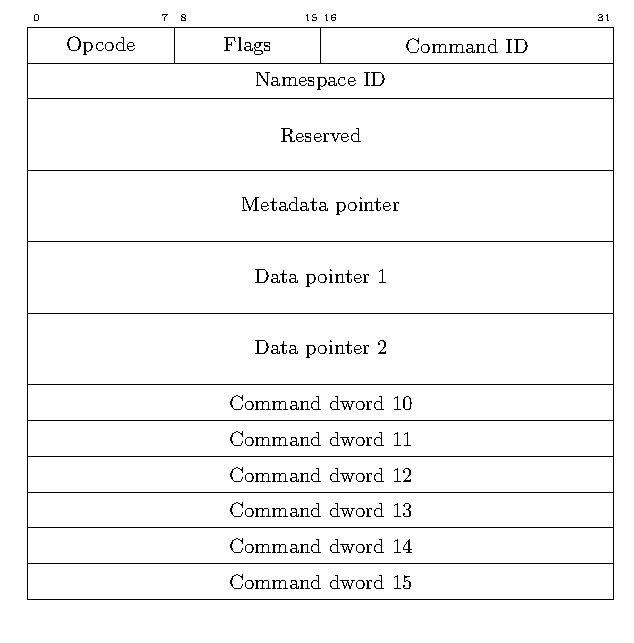
\includegraphics[width=0.69\textwidth]{nvme-command}};

    \coordinate (nvme-tl) at ($ (sub-entry.north west) + (0.49,-0.49) $);
    \coordinate (nvme-bl) at ($ (sub-entry.south west) + (0.49,0.70) $);
    \draw[line width=0.05mm, -] (a.three east) -- (nvme-tl);
    \draw[line width=0.05mm, -] (a.three east) -- (nvme-bl);

  \end{tikzpicture}
\end{document}

